\subsection{Getting Started with the FFW}
\label{sect:QuickStart:gettingStarted}

\noindent This subsection will describe how to execute an existing script for a problem and how to manipulate it.\medskip

\noindent In the following we are interested in the solution $u$ of the elliptic PDE
\begin{align*}
- \ddiv (\kappa \,\grad u) + \lambda \,\grad u + \mu \, u &= f &&\text{in } \Omega,\\
u &= u_D &&\text{on } \Gamma,\\
\frac{\partial u}{\partial n} &= g &&\text{on } \partial\Omega \setminus \Gamma.
\end{align*}
As model problem we consider the above problem with $\kappa = I$, $\lambda = 0$, $\mu = 0$, $f \equiv 1$, $u_D \equiv 0$ and $g \equiv 0$, on a L-shaped domain $\Omega$ with Dirichlet boundary only (Neumann boundary $\partial\Omega \setminus \Gamma = \emptyset$).\medskip

\noindent The script \code{gettingStarted.m} in the root folder shows the basic usage of the \FFW\!. It's code is printed in Figure~\ref{sect:Quickstart.fig.code:gettingStarted}.

\begin{figure}[ht!]
%\inputcoden{../gettingStarted.m}
\begin{pcoden}
function p = gettingStarted

problem = 'Elliptic_Lshape';
pdeSolver = 'P1';
maxNrDoF = 100;
mark = 'bulk';

p = initFFW(pdeSolver,problem,mark,maxNrDoF,'elliptic');
p = computeSolution(p);

figure(1);
set(gcf,'Name','Displacement');
p = show('drawU',p);
view(-30,20)

figure(2);
set(gcf,'Name','Estimated Error');
p = show('drawError_estimatedError',p);
\end{pcoden}

\caption{Content of \code{gettingStarted.m}}\label{sect:Quickstart.fig.code:gettingStarted}
\end{figure}

\medskip
\noindent To start the script, set MATLAB's current directory to the root of the \FFW and execute it.\medskip

\noindent 
\begin{enumerate}[{\hspace{15mm}}]
\item[Line 3:] The name of a file that describes the problem definition. This file is located at \path{.\problems\elliptic\}. For more details on the geometry refer to Section~\ref{sect:DataStructures}. For more details on the problem definition see also Subsection~\ref{sect:QuickStart:ProblemDefinition}.
\item[Line 4:] The type of finite element method is chosen. This can possibly also be \code{'CR'}.
\item[Line 5:] This is the indicator when to stop the refinement, i.e., the calculations. For more details refer to Section~\ref{sect:MeshGeneration}.
\item[Line 6:] The mark algorithm is chosen. The argument can also be \code{'maximum'} or \code{'uniform'}. For more details refer to Section~\ref{sect:MeshGeneration}.
\item[Line 8:] The \FFW is initialized with the above arguments, i.e., the structure \code{p} is created. The last argument describes what problem type is to be computed. This argument can possibly also be \code{'elasticity'}. See also Section~\ref{sect:ImplementedProblems}.
\item[Line 9:] The actual calculations are started. See also Section~\ref{sect:FlowChart} for details.
\item[Line 12:] The solution is plotted with the standard parameters. More details about the \code{show} function as well as its parameters can be found in Section~\ref{sect:GraphicalOutput}.
\item[Line 15:] The estimated error is plotted with the standard parameters.
\end{enumerate}
\bigskip

\noindent For the results, i.e. the solution and the estimated error, of the \code{gettingStarted.m} script, see Figure~\ref{sect:Quickstart.fig.plots.gettingStarted}.

\begin{figure}[ht!]
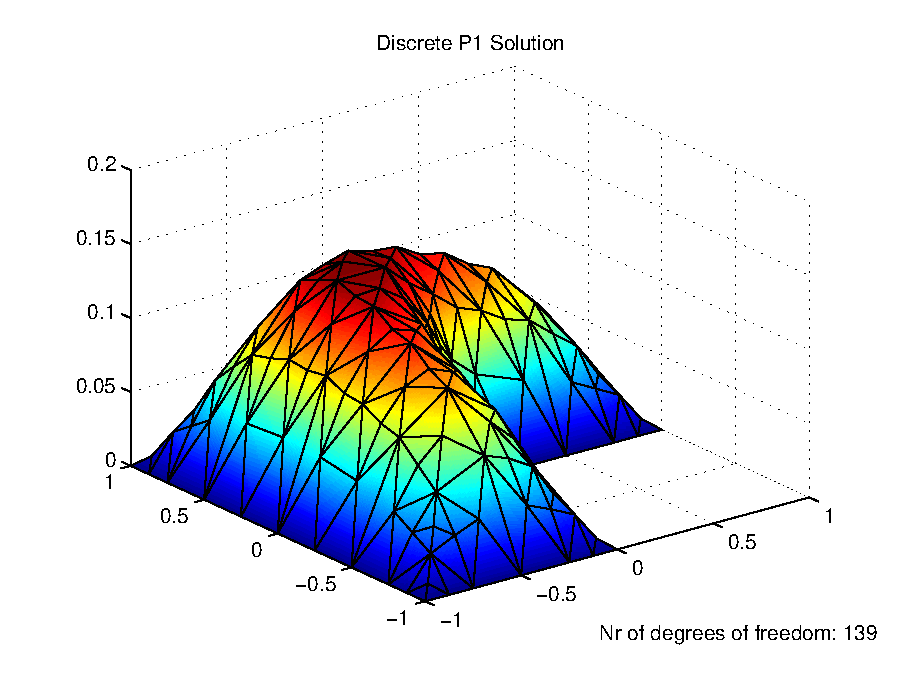
\includegraphics[width= 0.49\textwidth]{images/sect_QuickStart_LShapeU1}
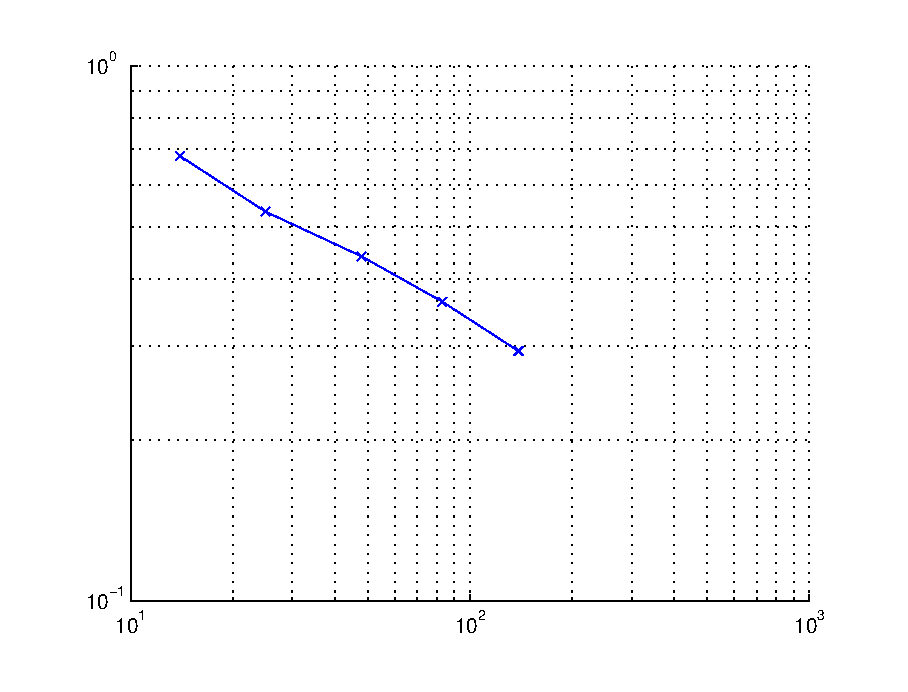
\includegraphics[width= 0.49\textwidth]{images/sect_QuickStart_LShapeE1}\\
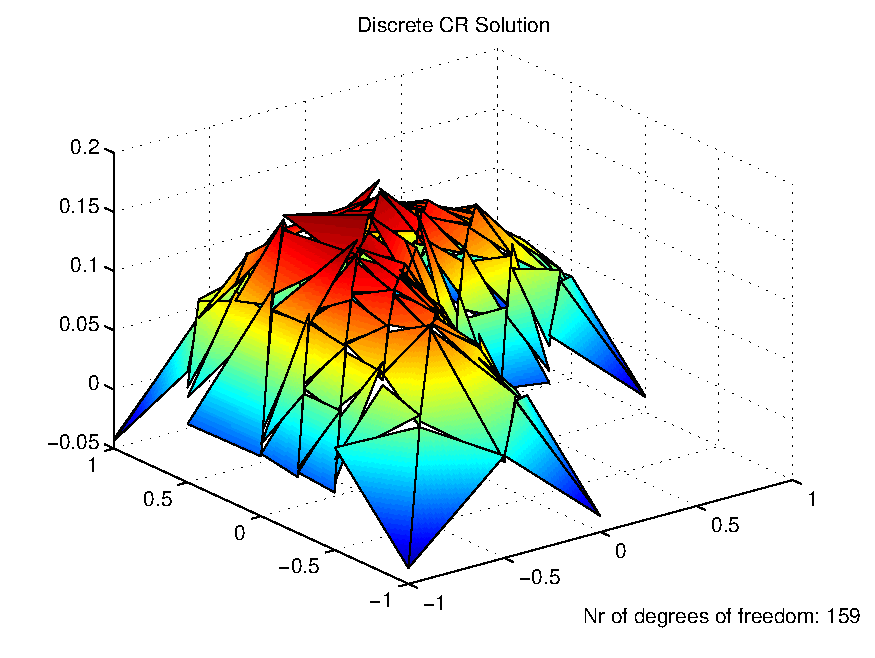
\includegraphics[width= 0.49\textwidth]{images/sect_QuickStart_LShapeU2}
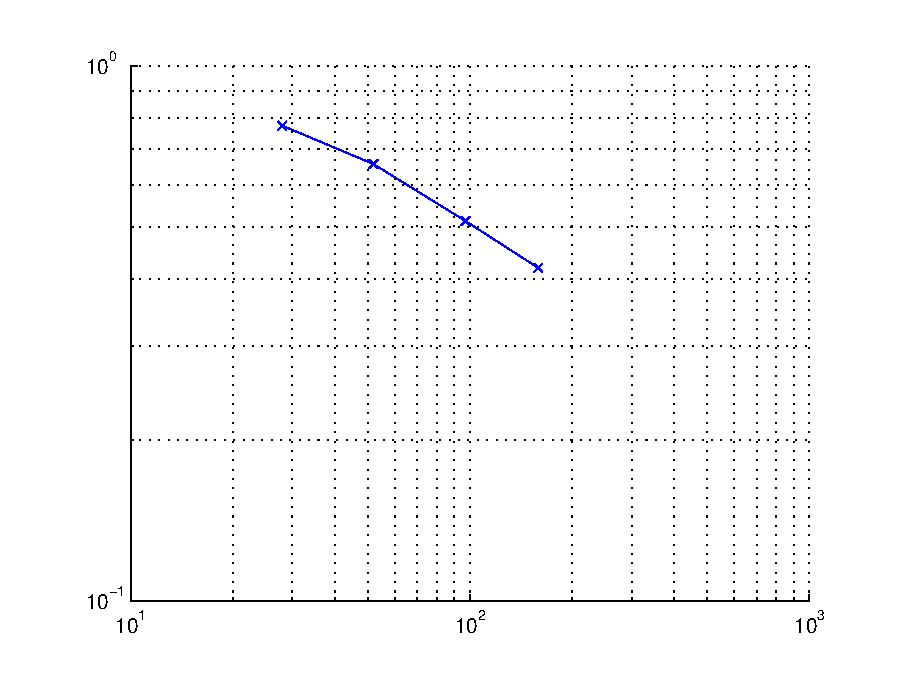
\includegraphics[width= 0.49\textwidth]{images/sect_QuickStart_LShapeE2}
\caption{Plots obtained from the \code{gettingStarted.m} script for \code{pdeSolver = 'P1'} on top and \code{pdeSolver = 'CR'} below.}\label{sect:Quickstart.fig.plots.gettingStarted}
\end{figure}

\clearpage
